\documentclass[a4paper,12pt,twoside]{article}

\usepackage[ngerman,english]{babel}

%%% FOR DISPLAYING CODE
\usepackage[procnames]{listings}
\usepackage{xcolor}

%%% MARGINS
\usepackage{geometry}
% INFO: https://www.overleaf.com/learn/latex/Page_size_and_margins
\geometry{
	a4paper,
%	total={170mm,257mm},
	left=25mm,
	top=25mm,
	textwidth=16cm,
	textheight=23cm,
%	right=25mm,
%	bottom=40mm,
}

%%% SPACING
%\usepackage{setspace} 
%\onehalfspacing

\usepackage{siunitx} % for writing numbers with units % e.g. \SI{6.3e8}{km}, \ang{62.59}, \num{100}'s \si{km}, \SI{53}{\degree}
\usepackage{amsmath,amssymb}
\usepackage{graphicx}
\usepackage{datetime} 
\usepackage{color}
\usepackage{float} %without it, tables position more or less random, with this an writing \begin{table}[H] the table appears right where it is defined!
\usepackage{mathptmx}
\usepackage{enumitem}

\usepackage[T1]{fontenc}
\usepackage[utf8]{inputenc}

\usepackage{pgfplots} % for plotting functions
\pgfplotsset{compat=1.16}

%%% HEADER and FOOTER
%\usepackage[automark,headsepline]{scrpage2}
%\ihead[]{\headmark}
%\chead[]{}
%\ohead[]{\pagemark}
%\ifoot[]{}
%\cfoot[\pagemark]{}
%\ofoot[]{}
%\pagestyle{scrheadings}

\usepackage{lipsum}

%% LINE SPACING
\usepackage{setspace}
\setstretch{1.5}

%%% HYPERLINKS
\usepackage{hyperref} % muss sich vor cite stuff befinden

%% SET IMAGE PATH (where images are stored)
\graphicspath{{figures/}}

%%% CITE
\usepackage{apacite}
\bibliographystyle{apacite}

%!TEX root = ../maturaarbeit.tex

%%%%%%%%%%%%%%%%%%%%%%%%%%%%%%%%%%
% DEFINE COLORS
\definecolor{red}{rgb}{0.6,0,0} 
\definecolor{blue}{rgb}{0,0,0.6}
\definecolor{green}{rgb}{0,0.8,0}
\definecolor{cyan}{rgb}{0.0,0.6,0.6}

\definecolor{mypink}{rgb}{0.753,0.000,0.890}
\definecolor{myblue}{rgb}{0.078,0.000,1.000}
\definecolor{mybluedark}{rgb}{0.004,0.024,0.525} \definecolor{mygreen}{rgb}{0.000,0.514,0.000}
\definecolor{myreddark}{rgb}{0.698,0.000,0.008}
\definecolor{mycyan}{rgb}{0.000,0.506,0.612}
\definecolor{mybrown}{rgb}{0.494,0.365,0.090}

%%% DISPLAY CODE
\usepackage{listings}
\newcommand\pythonstyle{\lstset{
    language=Python,
	tabsize=4,
	basicstyle=\normalsize\sffamily,
	numberstyle=\color{gray},
	stringstyle=\color{myreddark},
    commentstyle=\color{mygreen},
    % KEYWORDS
    % main keywords
	keywordstyle=\normalsize\color{myblue},%\bfseries,
    % add keywords (main blue)
    emph={False,None,True,self,TODO},
    emphstyle={\color{myblue}},
    % pink emph
    emph={[2]assert,break,continue,del,elif ,else,except,finally,for,from,global,if,import,in,pass,raise,return,try,while,with,yield},
    emphstyle={[2]\color{mypink}},%\bfseries,
    %dark blue emph
    emph={[3]execfile,reduce,xrange},
    emphstyle={[3]\color{mybluedark}},
    % brown emph
    emph={[4]exec,print,isinstance,zip,enumerate,reversed,len,repr},
    emphstyle={[4]\color{mybrown}},
    % cyan emph
    emph={[5]object,type,list,set,dict,tuple,str,super},
    emphstyle={[5]\color{mycyan}},
    % errors (also cyan emph)
    emph={[6]Exception,NameError,IndexError,SyntaxError,TypeError,ValueError,OverflowError,ZeroDivisionError},
    emphstyle={[6]\color{mycyan}},
    % errors (also cyan emph)
    emph={[7]copy,deepcopy,append,real,imag},
    emphstyle={[7]\color{black}},
    % 
    showstringspaces=false,
	breaklines=true,
	numbers=left,
    frame=tb,
	xleftmargin=15pt
}}

\newcommand\javascriptstyle{\lstset{
	basicstyle=\small\sffamily,
    keywordstyle=\color{blue}\bfseries,
    commentstyle=\color{purple}\ttfamily,
    stringstyle=\color{red}\ttfamily,
	numberstyle=\color{gray},
    keywords={typeof, new, true, false, catch, function, return, null, catch, switch, var, if, in, while, do, else, case, break},
    ndkeywords={class, export, boolean, throw, implements, import, this},
    ndkeywordstyle=\color{darkgray}\bfseries,
    identifierstyle=\color{black},
    comment=[l]{//},
    morecomment=[s]{/*}{*/},
    morestring=[b]',
    morestring=[b]",
    showstringspaces=false,
	breaklines=true,
	numbers=left,
    frame=tb,
	xleftmargin=15pt,
    sensitive=false,
}}

\newcommand\csharpstyle{\lstset{
	language=csh,
	tabsize=4,
	basicstyle=\small\sffamily,
	numberstyle=\color{gray},
	stringstyle=\color{myreddark},
    commentstyle=\color{mygreen},
	morecomment=[l]{//}, %use comment-line-style!
	morecomment=[s]{/*}{*/}, %for multiline comments
    % KEYWORDS
	keywordstyle=\normalsize\color{myblue},%\bfseries,
	morekeywords={ abstract, event, new, struct,
		as, explicit, null, switch,
		base, extern, object, this,
		bool, false, operator, throw,
		break, finally, out, true,
		byte, fixed, override, try,
		case, float, params, typeof,
		catch, for, private, uint,
		char, foreach, protected, ulong,
		checked, goto, public, unchecked,
		class, if, readonly, unsafe,
		const, implicit, ref, ushort,
		continue, in, return, using,
		decimal, int, sbyte, virtual,
		default, interface, sealed, volatile,
		delegate, internal, short, void,
		do, is, sizeof, while,
		double, lock, stackalloc,
		else, long, static,
		enum, namespace, string},
	% 
    showstringspaces=false,
	breaklines=true,
	numbers=left,
    frame=tb,
	xleftmargin=15pt	
}}

% Python environment
\lstnewenvironment{python}[1][]
{
	\pythonstyle
	\lstset{#1}
}
{}
\lstnewenvironment{javascript}[1][]
{
	\javascriptstyle
	\lstset{#1}
}
{}
\lstnewenvironment{csharp}[1][]
{
	\csharpstyle
	\lstset{#1}
}
{}

% CODE FOR EXTERNAL FILES
\newcommand\pythonexternal[2][]{{
		\pythonstyle
		\lstinputlisting[#1]{#2}}}

% CODE FOR INLINE
\newcommand\pythoninline[1]{{\pythonstyle\lstinline!#1!}}
\newcommand\csharpinline[1]{{\csharpstyle\lstinline!#1!}}
\newcommand\javascriptinline[1]{{\javascriptstyle\lstinline!#1!}}

%% DEFINE CUSTOM COMMANDS AND SHORTCUTS

% some commands
\def\ba#1\ea{\begin{align}#1\end{align}}
\def\bas#1\eas{\begin{align*}#1\end{align*}}
\def\bmat#1\emat{\begin{pmatrix}#1\end{pmatrix}}
\newcommand{\ve}[1]{\vec{#1}}
\newcommand{\veTwo}[2]{\begin{pmatrix}#1\\#2\end{pmatrix}}
\newcommand{\veThree}[3]{\begin{pmatrix}#1\\#2\\#3\end{pmatrix}}
\newcommand{\veFour}[4]{\begin{pmatrix}#1\\#2\\#3\\#4\end{pmatrix}}
\newcommand{\ora}[1]{\overrightarrow{#1}}
\newcommand{\ola}[1]{\overleftarrow{#1}}
\newcommand{\s}[1]{\sqrt{#1}}

\def \bit{\begin{itemize}\setlength\itemsep{0em}} %\vspace{-5mm}
	\def \eit{\end{itemize}}

\def \ben{\begin{enumerate}\setlength\itemsep{0em}} %\vspace{-5mm}
	\def \een{\end{enumerate}}

\def \N{\mathbb{N}}
\def \Z{\mathbb{Z}}
\def \Q{\mathbb{Q}}
\def \R{\mathbb{R}}
\def \C{\mathbb{C}}

\def \ra{\rightarrow}
\def \longra{\longrightarrow}
\def \Ra{\Rightarrow}
\def \Longra{\Longrightarrow}
\def \la{\leftarrow}
\def \longla{\longleftarrow}
\def \La{\Leftarrow}
\def \Longla{\Longleftarrow}

\def \lra{\leftrightarrow}
\def \longlra{\longleftrightarrow}
\def \Lra{\Leftrightarrow}
\def \Longlra{\Longleftrightarrow}

\def \l{\left}
\def \r{\right}

\def \a{\alpha}
\def \b{\beta}
\def \g{\gamma}

\def \c{\cdot}

\def \el{\in}
\def \notel{\notin}

\newcommand{\f}{\frac}

\def \q{\quad}
\newcommand{\p}{\phantom}

\def\bs#1\es{\begin{split}#1\end{split}}


\def \L{\mathbb{L}}




\begin{document}

%%%%%%%%%%%%%%%%%%%%%%%%%%%%%%%%%%%%%%%%%%%%%%%%%%%%%%%
%%%%%%%%%%%%%%%%%%%%%%%%%%%%%%%%%%%%%%%%%%%%%%%%%%%%%%%
%%%%%%%%%%%%%%%%%%%%%%%%%%%%%%%%%%%%%%%%%%%%%%%%%%%%%%%

%%% AB HIER ARBEITEN, WEITER OBEN NICHTS VERAENDERN
%%% Ausnahme: Einbinden weitere Pakete

\selectlanguage{ngerman} %% HIER SPRACHE EINSTELLEN! english, ngerman

\begin{titlepage}
	\clearpage\thispagestyle{empty}	
	\setstretch{1}
	
	\begin{minipage}[t]{\textwidth}
		\begin{minipage}[t]{0.5\textwidth}
			Max Muster\\
			Musterstrasse 3a\\
			1234 Musterdorf\\
			079 123 45 67\\
			max@muster.com
		\end{minipage}
		\begin{minipage}[t]{0.5\textwidth}
			\begin{flushright}
				Kantonsschule Romanshorn\\
				Klasse 4M???\\
				Maturaarbeit
			\end{flushright}
		\end{minipage}
	\end{minipage}
	
	\vspace{4cm}
	
	{
		\centering
		\Huge\bfseries Titel meiner Arbeit\par
		\vspace{1cm}
		\includegraphics[width=0.15\textwidth]{example-image-1x1}\par
	}
	
	\vspace{9cm}	
	\noindent
	Fach: ??? \noindent\\
	Betreuungsperson: Dr. Andreas Schärer\\
	Abgabetermin: ?? ????? 20??
	
\end{titlepage}

%%%%%%%%%%%%%%%%%%%%%%%%%%%%%%%%%%%%%%%%%%%%%%%%%%%%%%%
%%%%%%%%%%%%%%%%%%%%%%%%%%%%%%%%%%%%%%%%%%%%%%%%%%%%%%%
%%%%%%%%%%%%%%%%%%%%%%%%%%%%%%%%%%%%%%%%%%%%%%%%%%%%%%%

% \null\thispagestyle{empty}\clearpage

%%% ABSTRACT

\pagenumbering{roman}

\section*{Abstract}

Im Abstract wird das Wichtigste in aller Kürze zusammengefasst. Typischerweise besteht er aus ca. $1/4$-Seite.

%%%%%%%%%%%%%%%%%%%%%%%%%%%%%%%%%%%%%%%%%%%%%%%%%%%%%%%
%%%%%%%%%%%%%%%%%%%%%%%%%%%%%%%%%%%%%%%%%%%%%%%%%%%%%%%
%%%%%%%%%%%%%%%%%%%%%%%%%%%%%%%%%%%%%%%%%%%%%%%%%%%%%%%

%%% TABLE OF CONTENTS

%\null\thispagestyle{empty}\clearpage
\newpage
%\setcounter{page}{1}
\tableofcontents

\parindent=0pt
\parskip=6pt

\newpage

\pagenumbering{arabic}

%%%%%%%%%%%%%%%%%%%%%%%%%%%%%%%%%%%%%%%%%%%%%%%%%%%%%%%
%%%%%%%%%%%%%%%%%%%%%%%%%%%%%%%%%%%%%%%%%%%%%%%%%%%%%%%
%%%%%%%%%%%%%%%%%%%%%%%%%%%%%%%%%%%%%%%%%%%%%%%%%%%%%%%

\section{Einleitung}

Hier kommt die Einleitung. Wichtig: Auf Leitfrage der Arbeit eingehen!

%%%%%%%%%%%%%%%%%%%%%%%%%%%%%%%%%%%%%%%%%%%%%%%%%%%%%%%
%%%%%%%%%%%%%%%%%%%%%%%%%%%%%%%%%%%%%%%%%%%%%%%%%%%%%%%
%%%%%%%%%%%%%%%%%%%%%%%%%%%%%%%%%%%%%%%%%%%%%%%%%%%%%%%

\newpage
\section{Grundlagen von LaTeX}


\subsection{LaTeX einrichten}

\begin{enumerate}
    \item \textbf{LaTeX} installieren:
    \begin{itemize}
        \item Windows: \url{https://www.tug.org/texlive/windows.html}\\(klicke aus `install-tl-windows.exe')
        \item Mac \url{https://www.tug.org/mactex/mactex-download.html}\\(klicke auf `MacTeX.pkg.')
    \end{itemize}
    \item \textbf{Visual Studio Code} (kurz: VSCode, Editor) installieren:\\ \url{https://code.visualstudio.com}
    \item \textbf{LaTeX-Workshop-Extension} für VSCode installieren:
    \begin{figure}[H]
		\centering
		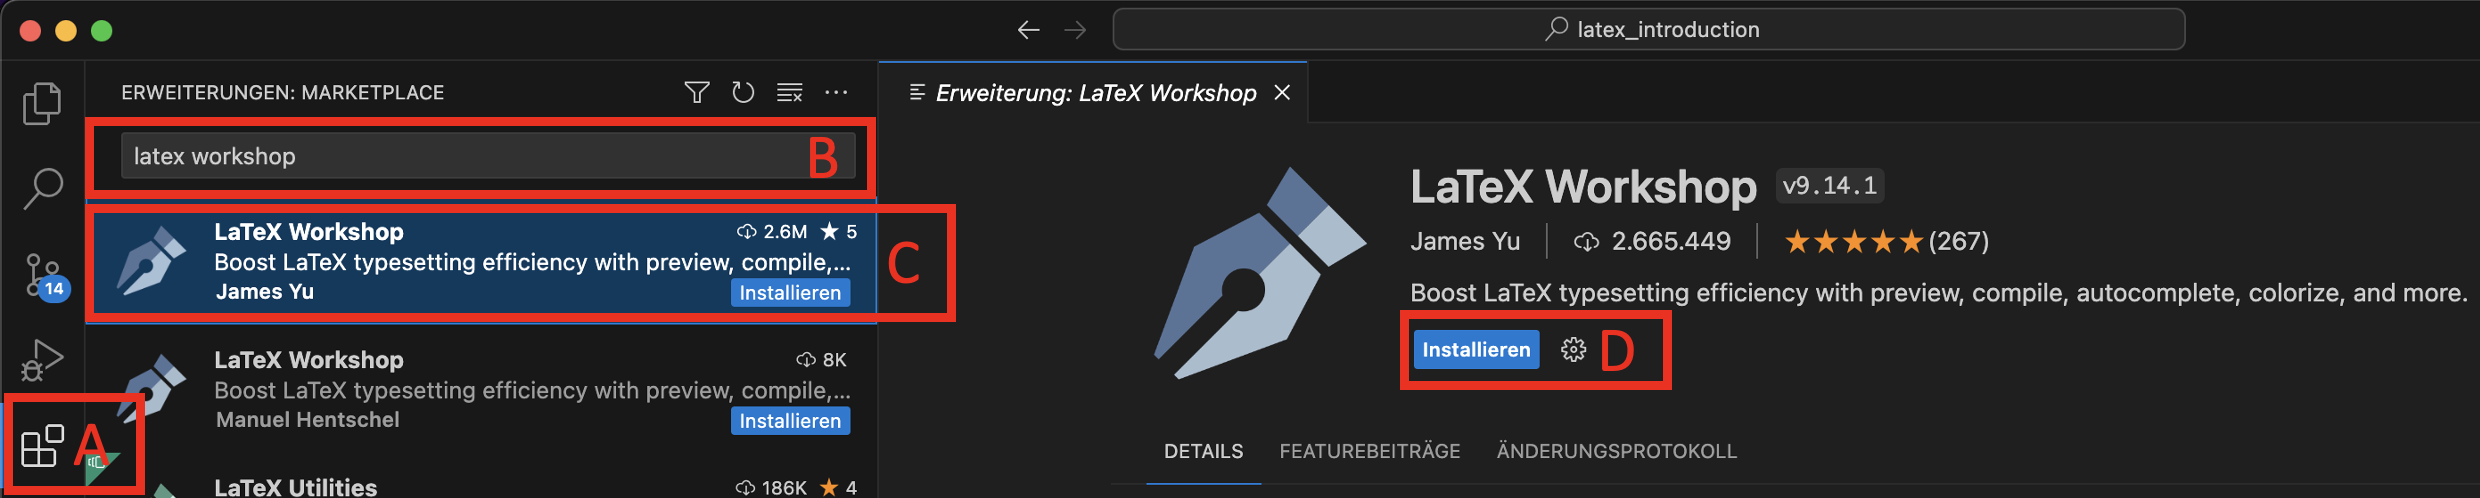
\includegraphics[width=\textwidth]{latex_workshop}
	\end{figure}
\end{enumerate}

\subsection{Erste Schritte mit LaTeX}

\begin{enumerate}
	\item Entzippe den Ordner mit dem Template und verschiebe diesen an einen passenden Speicherort.
	\item Öffne den Ordner in VSCode:
	\begin{enumerate}
		\item  VSCode öffnen
		\item  Datei / Ordner öffnen / Ordner auswählen
	\end{enumerate}
	\item Auf der linken Seite sollte nun der Inhalt des ganzen Ordners angezeigt werden.
	\item Das wichtigste File ist **"main.tex"**. Dieses kannst du passende umbenennen (z.B: "maturaarbeit.tex", "sla.tex" oder ...).
	\item Öffne nun das File: In dieses schreibst du den Inhalt deiner Arbeit. Nehme Änderungen vor.
	\item TeX-File \textbf{Kompilieren}:
	\begin{itemize}
		\item Nun muss das File kompiliert, also in ein PDF umgewandelt, werden.
		\item Dies sollte immer geschehen, wenn du speicherst.
		\item Alternativ kann man auch manuell kompilieren:
		\begin{enumerate}
			\item Command palette öffnen: Ctrl + Shift + P (Win), Shift + Command + P (Mac)
			\item "LaTeX Workshop: Build with recipe"
			\item "latexmk" oder "pdflatex -> bibtex -> pdflatex x2" (falls Quellen nicht richtig kompiliert werden)
		\end{enumerate}
	\end{itemize}
\end{enumerate}

\subsection{Sprachkorrektur}

Die Sprachkorrektur in VSCode ist leider nicht so gut. Verwende deshalb andere entsprechende Online-Tools. Man kann auch den Text in Work kopieren und die dortige Korrekturfunktion verwenden.

\subsection{Zitieren und Fussnoten}

Typischerweise gibt man direkt dort, wo man Information\footnote{in \textit{eigenen} Worten} wiedergibt, welche man in einer Quelle gefunden hat, die Quelle an~\cite{Aabkabla2019}. Das Tilde-Symbol for dem Zitierbefehl sorgt dafür, dass dort kein Zeilenumbruch gemacht wird. Falls der ganze Paragraph auf einer Quelle basiert, gibt man diese am Ende des Paragraphen an~\cite{Lamport1986,Ellwanger2015}.

\subsection{Nonsense Text}

Möchte man schnell viel Text generieren, kann wie folgt Text in der Nonsensesprache Lorem Ipsum einfügen:

\lipsum[1]

\section{Formeln und Grafiken}

\subsection{Mathematische Ausdrücke}

Mathematische Ausdrücke wie $f(x) = x^2$ kann man direkt im Fliesstext darstellen. Soll ein mathematischer Ausdruck aus einer eignen Linie stehen, verwendet man die \textit{equation-}Umgebgung:
\begin{equation}
	\label{equ name der funktion 1} % give the expression a name, use it to refer to this function.
	f(x) = \frac{x^3}{2} + 3 \,. % the \, adds a spacing before the full stop
\end{equation}
Dieser Ausdruck hat eine Nummer erhalten. Um auf einen math. Ausdruck zu verweisen, füge \textbf{niemals} eine \textit{harte}\footnote{Von Hand die entsprechende Nummer eingeben. Wenn sich nun die Nummerierung der Formel ändert, muss man von Hand alle harten Referenzen anpassen.} Referenz ein, sondern eine \textit{weiche}\footnote{Mit \textit{eqref}.}:
Die Funktion, die in Gleichung \eqref{equ name der funktion 1} gegeben ist, ist meine Lieblingsfunktion!

Möchte man nicht, dass eine Formel nummeriert ist, so fügt man einen \* im TeX-Code hinzu
\begin{equation*}
f(x) = \sin^2{(2\alpha)} + 3 \,.
\end{equation*}
Für mehrzeilige Rechnungen (mit oder ohne Nummer) verwendet man die \textit{align}-Umgebgung:
\begin{align*}
	0 &= ax^2 + bx + c \\
	x_{1,2} &= \frac{-b \pm \sqrt{b^2 - 4ac}}{2a}
\end{align*}
Mit dem \&-Symbol kann man die einzelnen Zeilen ausrichten.

Einfach weil wir können, fügen wir mit \textit{newpage} einen Seitenumbruch ein.

\subsection{Grafiken}

Graphen von Funktionen können direkt im tex-File gezeichnet werden:
\begin{figure}[H]
	\centering
	\begin{tikzpicture}[scale=1]
		\begin{axis}[
			axis x line=center,
			axis y line=center,
			yticklabel style = {font=\footnotesize, xshift=0.2ex},
			xticklabel style = {font=\footnotesize, yshift=0.2ex},
			xtick={-7,...,7},
			ytick={-7,...,7},
			xlabel={$x$},ylabel={$f(x)$},
			xlabel style={right},
			ylabel style={above},
			xmin=-7,xmax=8,ymin=-5,ymax=5,
			grid=both,
			grid style={line width=.1pt, draw=gray!10},
			major grid style={line width=.2pt,dashed, draw=gray!50},
			scale=1.5,
			unit vector ratio=1 1 1
			]
			\addplot[samples=501,domain=-7:7,magenta,ultra thick] plot ({x},{x*sin(x*360/(2*pi))}) node[above,pos=0.58] {$\small{f(x)=x\cdot\sin{x}}$};
		\end{axis}
	\end{tikzpicture}
\end{figure}


%%%%%%%%%%%%%%%%%%%%%%%%%%%%%%%%%%%%%%%%%%%%%%%%%%%%%%%

\newpage
\section{Bilder, Listen und Aufzählungen}

\subsection{Bilder einfügen}

Soll ein Bild eingefügt werden, so wird es im entsprechenden Ordner abgelegt. Nachher kann über den Namen des Bilds auf dieses zugegriffen werden:
\begin{figure}[H]
	\centering
	
\includegraphics[width=0.4\textwidth]{grumpy_cat}
	\caption[Eintrag in Abbildungsverzeichnis von Grumpy Cat]{Grumpy cat. The Grumpy Cat is a grumpy cat.}
	\label{fig grumpy cat.}
\end{figure}
Natürlich kann man auch Referenzen auf Bilder einfügen. Bild \ref{fig grumpy cat.} zeigt die Grumpy Cat. Die Breite/Höhe eines Bildes kann man angeben z.B. mit width=3cm oder height=15mm.
Soll das Bild die halbe Breite des Textes haben, kann man angeben
width=0.5\textbackslash textwidth

\subsection{Listen und Aufzählungen}

Eine Liste generiert man wie folgt:
\begin{itemize}
	\item Erstes Element
	\item Zweites Element
	\item Drittes Element
	\item Viertes Element
\end{itemize}

Eine sehr kompakte Liste so:
\begin{itemize}
	\vspace{-\topsep}
	\setlength{\itemsep}{0pt}\setlength{\parskip}{0pt}
	\item Erstes Element
	\item Zweites Element
	\item Drittes Element
	\item Viertes Element
\end{itemize}

\subsection{Aufzählung}

Aufzählung mit Zahlen nummeriert:
\begin{enumerate}
	\item Erstes Element
	\item Zweites Element
	\item Drittes Element
	\item Viertes Element
\end{enumerate}

Aufzählung mit Grossbuchstaben nummeriert:
\begin{enumerate}[label=\Alph*]
	\item Erstes Element
	\item Zweites Element
	\item Drittes Element
	\item Viertes Element
\end{enumerate}

Aufzählung mit krossbuchstaben nummeriert:
\begin{enumerate}[label=\alph*)]
	\item Erstes Element
	\item Zweites Element
	\item Drittes Element
	\item Viertes Element
\end{enumerate}

Aufzählung mit römischen Buchstaben nummeriert:
\begin{enumerate}[label=(\roman*)]
	\item Erstes Element
	\item Zweites Element
	\item Drittes Element
	\item Viertes Element
\end{enumerate}

\subsection*{Kapitel ohne Nummerierung}

Wer die Nummer von diesem Kapitel findet, soll sich bitte direkt beim Kapitel melden!

\newpage

\section{Tabellen und Symbole}

\subsection{Tabelle}

Tatsächlich ist es einigermassen mühsam, Tabellen zu erstellen:
\begin{table}[H]
	\centering
	\renewcommand{\arraystretch}{1.5}
	\begin{tabular}{|>{\centering\arraybackslash}p{7cm}|>{\centering\arraybackslash}p{7cm}|}
	\hline
	x & y \\ \hline
	4 & 2\\ \hline
	\end{tabular}
	%\caption{}
	%\label{tab }
\end{table}

Verwende den folgenden Tabellen-Generator, um einfache Tabellen zu erzeugen: \url{https://www.tablesgenerator.com}

\subsection{Symbole}

Falls du nicht weisst, wie man ein gewisses Symbol in LaTeX darstellst, so hilft dir folgende Seite, um dieses zu identifizieren: \url{http://detexify.kirelabs.org/classify.html}

%%%%%%%%%%%%%%%%%%%%%%%%%%%%%%%%%%%%%%%%%%%%%%%%%%%%%%%

\newpage
\section{Code}

\subsection{Python Code}

Code-Ausschnitt:

\begin{python}
import numpy as np

print("Hello World")

for i in range(3):
	print(i)
\end{python}

Code direkt im Fliesstext integriert: \pythoninline{print(42)}.

\subsection{JavaScript and TypeScript Code}

\begin{javascript}
function greeter(person: string) {
	return "Hello, " + person;
} 

let user = "Jane User";

document.body.textContent = greeter(user);
\end{javascript}

Code direkt im Fliesstext integriert: \javascriptinline{let user = "Jane User";}.


\subsection{C\# Code}

\begin{csharp}
using System;

namespace HelloWorld
{
  class Program
  {
    static void Main(string[] args)
    {
      Console.WriteLine("Hello World!");    
    }
  }
}
\end{csharp}

Code direkt im Fliesstext integriert: \csharpinline{Console.WriteLine("Hello World!");}.

%%%%%%%%%%%%%%%%%%%%%%%%%%%%%%%%%%%%%%%%%%%%%%%%%%%%%%%

\newpage
\appendix

\section{Erster Anhang}

Ergänzende Informationen gehören in den Anhang. Wären diese Informationen im Haupttext der Arbeit, würden sie stören, zum Beispiel weil es zu viel und zu detailliert ist. In den Anhang (unter Umständen) gehören:
\begin{itemize}
	\item Code einer Programmierarbeit (Zeige im Haupttext nur Codeausschnitte, die der Argumentation helfen)
	\item detaillierte Berechnungen
	\item Ergebnisse einer Umfrage
	\item Interviews
	\item \ldots
\end{itemize}

%%%%%%%%%%%%%%%%%%%%%%%%%%%%%%%%%%%%%%%%%%%%%%%%%%%%%%%

\newpage

\section{Zweiter Anhang}

Anhang der Zweite.


%%%%%%%%%%%%%%%%%%%%%%%%%%%%%%%%%%%%%%%%%%%%%%%%%%%%%%%
%%%%%%%%%%%%%%%%%%%%%%%%%%%%%%%%%%%%%%%%%%%%%%%%%%%%%%%
%%%%%%%%%%%%%%%%%%%%%%%%%%%%%%%%%%%%%%%%%%%%%%%%%%%%%%%

%%%%%%%% AB HIER NICHTS MERH VERAENDERN!

%%%%%%%%%%%%%%%%%%%%%%%%%%%%%%%%%%%%%%%%%%%%%%%%%%%%%%%
%%%%%%%%%%%%%%%%%%%%%%%%%%%%%%%%%%%%%%%%%%%%%%%%%%%%%%%
%%%%%%%%%%%%%%%%%%%%%%%%%%%%%%%%%%%%%%%%%%%%%%%%%%%%%%%

\newpage

\clearpage

\bibliography{biblio}

\newpage
\addcontentsline{toc}{section}{\listfigurename} % Fuege Abb.vz zu TOC hinzu
\listoffigures % Abbildungsverzeichnis


\end{document}

